\chapter{AM e Python}

A seguir um exemplo de modelo preditivo em Python. O modelo utiliza o algoritmo SVM e o conjunto de dados iris, que é um conjunto de dados conhecido e bastante utilizado como em demonstrações em outros livros e sites.

\begin{lstlisting}[language=Python, caption={Exemplo de código que usa AM}]
	from sklearn import svm
	from sklearn.datasets import iris
	iris = load_iris()
	X = iris.data
	y = iris.target
	model = svm.SVC()
	model.fit(X, y)
	model.predict([[2., 2., 2., 2.]])
\end{lstlisting}

\chapter{Estatística Básica}

Um conjunto de dados (geralmente para fins de análise) é organizado em uma estrutura tabular no formato de linhas e colunas. Cada coluna é chamado de atributo ou variável e cada linha é chamada de observação, ou registro, ou instância.

A Tabela~\ref{tbl:cliente} apresenta um exemplo de conjunto de dados com dados de clientes. A primeira linha da tabela define o nome dos atributos, são eles: \textit{Nome}, \textit{Endereço}, \textit{Telefone}, \textit{Salario}, e \textit{Concede crédito}; cada linha abaixo do nome da coluna representa um cliente. %Portanto a primeira linha tem o nome das colunas; a segunda linha tem dados de um determinado cliente, e a terceira linha dados de outro cliente.

\begin{table}
	\centering
	\caption{Tabela cliente.}
	\begin{tabular}{|l|l|c|l|c|}
	\hline
	\textbf{Nome} & \textbf{Endereço} & \textbf{Telefone} & \textbf{Salario} & \textbf{Concede crédito}\\
	\hline
	Jose Carlos & Rua das alamedas[...] & 222 96666 & 1.000,00 & Sim \\
	\hline
	Alex Borges & Avenida Fernandes[...]& 333 96589 & 2.000,00 & Não\\
	\hline
	\end{tabular}
	\label{tbl:cliente}
\end{table}

%A Tabela~\ref{tbl:cliente} apresenta dois clientes. Cada linha são dados relacionados a um determinado cliente.

%A primeira coluna é uma descrição das informações que existirão naquela coluna, por exemplo \textit{Nome} significa que todos os dados dessa coluna são referentes ao nome de determinado cliente. já cada linha abaixo da primeira linha são os dados propriamente ditos do cliente em específico.

Para apresentar uma estatística de resumo (tais como, média, mediana ou moda) ou algum gráfico (por exemplo, de barras ou de linhas) temos que conhecer o tipo do atributo para podermos selecionar qual a técnica mais adequada que devemos aplicar. Por exemplo, não podemos calcular a média para todos os atributos do cliente. Qual é a média do nome? ou a média do endereço, ou a média do telefone? Não faz sentido a estatística média para estes atributos. Pode parecer óbvio para estes casos porém nem tanto para outros.

Utilizando uma classificação teórica para esse tipo de atributo, podemos definir qual é o tipo possível de operação. Portanto, vamos acrescentar mais uma informação (teórica) a coluna da tabela para que possamos claramente definir o que deve, ou pode ser feito com ela, chamamos essa informação de tipo de dado, ou tipo de variável, que é o termo mais usado.

Conhecendo estes tipo e sua aplicação correta não cometeremos o erro de por exemplo, calcular a média de uma variável do tipo qualitativa ordinal. Além disso, é interessante reportar nos estudos científicos (artigos) uma tabela com o tipo das variáveis utilizado, pois isso facilita muito o entendimento do conjunto dos dados para o leitor interessado, caso o artigo tenha utilizado um conjunto de dados.

\section{Resumo}

\begin{tcolorbox}
O objetivo é descrever a tipologia das variáveis para que possamos utilizar corretamente as técnicas estatísticas e de aprendizagem de máquina.
\end{tcolorbox}

\newpage

\section{Variável}

\begin{tcolorbox}[title=Tipos de variável]
Uma variável (ou atributo) pode ser de dois tipos, ou quantitativo (também chamado de métrico) ou qualitativo (também chamado de não métrico, ou categórico).
\end{tcolorbox}

\begin{tcolorbox}[title=Escalas da variável (Mensuração)]
Uma variável tem uma escala de mensuração.
\end{tcolorbox}

\begin{tcolorbox}[title=Escalas da variável (contagem ou categorização)]
Um variável tem uma escala ou de contagem ou de categorização. Se quantitativo de contagem; se qualitativo de categorização.
\end{tcolorbox}


Nesta seção utilizaremos o termo variável com o significado de atributo. A ciência de dados é uma área interdisciplinar e utiliza técnicas de estatística, computação e matemática. Em estatística, uma variável é uma característica do que foi observado em uma amostra. Essa mesma característica é chamado de parâmetro quando está relacionado a população. Já em computação variável tem uma outra conotação, é um espaço em memória que armazena um valor que pode ser digitado pelo usuário ou inicializado. Porém em análise de dados uma variável também é chamado de atributo, é este conceito que iremos utilizar.

%\begin{tcolorbox}[colframe=blue!50!black, colback=yellow!10!white, coltitle=red, title=Título da Caixa]
%Este é o texto dentro de uma caixa personalizada.
%\end{tcolorbox}

Uma variável (ou atributo) pode ser de alguma forma (a) mensurada. Além disso, ela ainda pode ser ou (b) contada ou (c) categorizada. Chamamos isso de escalas. Além destas três escalas, (a) mensuração, (b) contagem e (c) categorização, classificamos as variáveis em dois tipos, quantitativas ou numéricas, e qualitativas, ou não numéricas. Se a variável for quantitativa ela tem uma escala de contagem, se for qualitativa uma escala de categorização. Ambas tem obrigatoriamente uma escala de mensuração.

%[	sibling distance=10em,
%  	every node/.style =
%	{
%		shape=rectangle,
%		rounded corners,
%   	draw,
%		align=center,
%   	top color=white,
%		bottom color=blue!20
%	}
%]
%]

\begin{figure}[h]
	\centering
	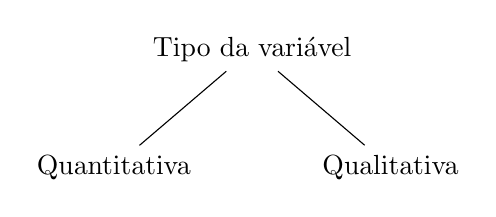
\begin{tikzpicture}[sibling distance=10em,]
	  \node {Tipo da variável}
	   child{node{Quantitativa}}
	   child{node{Qualitativa}};
	\end{tikzpicture}
	\label{fig:tipovariavel2}
\end{figure}

Na Tabela~\ref{tblstorypoint} as variáveis são: id, issuekey, title, descripton e storypoints. Elas foram registradas nessa tabela após os processos de mensuração, contagem ou categorização. %Por exemplo, medimos em story points o esforço para conclusão dessa User Story na coluna storypoints.

\newpage

É útil definir de qual tipo é determinada variável, pois, existem técnicas adequadas para cada tipo. Para realizar uma análise estatística descritiva, elaborar um gráfico para um artigo científico, ou aplicar uma técnica de pré-processamento em um modelo preditivo é necessário entender de qual tipo é cada variável e quais as suas escalas, pois existem determinadas técnicas para determinados fins. Por isso, vamos entender estas classificações teóricas.

Neste contexto, uma variável pode ser \textbf{quantitativa} ou \textbf{qualitativa} (Figura~\ref{fig:tipovariavel}). Além disso, uma variável quantitativa também é chamada de métrica, e a variável qualitativa de não métrica ou categórica \cite{favero2017manual}.



A variável quantitativa é expressa geralmente como um número. Porém, existem casos em que números também expressam variáveis qualitativas, logo cada caso deve ser analisado individualmente. Já a variável do tipo qualitativa está relacionado ao pertencimento do valor mensurado a um universo. Um exemplo de variável qualitativa é o estado civil do cliente, que pode ser solteiro ou casado. Para continuarmos, vamos atualizar nossa tabela de cliente com duas novas variáveis, estado civil e altura, assim teremos variáveis dos tipos qualitativa e quantitativas  na mesma tabela, o que é bem comum (Tabela~\ref{tbl:cliente_v2}).

\begin{figure}
	\begin{lstlisting}
	import pandas as pd
	df = pd.read_csv('7764.csv')
	df.head()
	\end{lstlisting}

	\begin{tabular}{clllll}
	\multicolumn{1}{l}{\textbf{id}} &
	\multicolumn{1}{l}{\textbf{issuekey}} &
	\multicolumn{1}{l}{\textbf{created}} &
	\multicolumn{1}{l}{\textbf{title}} &
	\multicolumn{1}{l}{\textbf{description}} &
	\multicolumn{1}{l}{\textbf{storypoints}} \\
	\textbf{0} &
	  29688087 &
	  2020-01-17 &
	  Update templates for website... &
	  Relates to \&232 and \#6109 Go... &
	  1 \\
	\textbf{1} &
	  29682716 &
	  2020-01-16 &
	  Make sure that we Capture  ... &
	  This was raised in the PM ... &
	  1 \\
	\textbf{2} &
	  29644971 &
	  2020-01-15 &
	  Propose new IA for Brand ... &
	  \#\# Goals\textbackslash{}nPropose new IA for... &
	  1 \\
	\textbf{3} &
	  29494181 &
	  2020-01-10 &
	  Cache `node\_modules` for ... &
	  \# UPDATE NOTE: This MR ... &
	  1 \\
	\textbf{4} &
	  29437529 &
	  2020-01-09 &
	  Disable all remaining unn ... &
	  Similar to new site... &
	  1
	\end{tabular}%
	\label{tblstorypoint}

\end{figure}

\begin{table}
	\centering
	\caption{Tabela cliente atualizada com novas colunas e novos registros.}
	\begin{tabular}{|l|l|c|c|c|}
	\hline
	\textbf{Nome} & \textbf{Endereço} & \textbf{Telefone} & \textbf{Estado civil} & \textbf{Altura} \\
	\hline
	Giseldo Neo & Rua das Alam[..] & 222 66666 & casado & 1,80\\
	\hline
	Alex Barros & Avenida Ferna[..]& 333 6589 & solteiro & 1,70 \\
	\hline
	Pedro Alves & Alameda dos Anj[..]& 888 5879 & casado & 1,50 \\
	\hline
	Miguel Peixoto & BR 259, trecho[..]&  & solteiro & 1,79 \\
	\hline
	\end{tabular}
	\label{tblcliente_v2}
\end{table}

Para exemplificar, tipificaremos (ou classificaremos) as variáveis (ou  características) que foram medidas, contadas (com determinado grau de precisão) ou categorizadas dos clientes em uma outra tabela para registrar estes dados sobre as variáveis (se quantitativo ou qualitativo). Veja na Tabela~\ref{tblclienteclassificacao} o resultado dessa tipificação, para cada variável informamos se a variável é qualitativa ou quantitativa na segunda coluna, já na primeira coluna temos o nome da variável.

\begin{table}
	\centering
	\caption{Tipo das variáveis da tabela cliente.}
	\begin{tabular}{|c|c|}
		\hline
		\textbf{Nome da variável} &\textbf{Tipo da variável} \\
		\hline
		Nome & qualitativa \\
		\hline
		Endereço & qualitativa \\
		\hline
		Telefone & qualitativa \\
		\hline
		Estado Civil & qualitativa \\
		\hline
		Altura & quantitativa \\
		\hline
	\end{tabular}
	\label{tblclienteclassificacao}
\end{table}

No entanto, ainda temos uma outra classificação das variáveis, relacionada as \textbf{escalas}. As escalas são 3: \textbf{mensuração}, \textbf{precisão} (da contagem) e \textbf{categorização}. As opções da escala mensuração são: \textbf{intervalar} e \textbf{razão} para as variáveis quantitativas e \textbf{nominal} e \textbf{ordinal} para as variáveis qualitativas. Veja na Figura~\ref{fig:escala}, o tipo das variáveis e as escalas de mensuração de cada tipo. Além das escalas de mensuração, temos as escalas de precisão e as escalas de categorização. A escala de precisão é utilizada somente nas variáveis quantitativas com as opções \textbf{discreta} ou \textbf{contínua}. Já a escala de categorização é utilizada somente em variáveis qualitativas, suas opções são \textbf{binária} ou \textbf{policotômica}.

\begin{figure}
	\caption{Escala da variável}
	\centering
	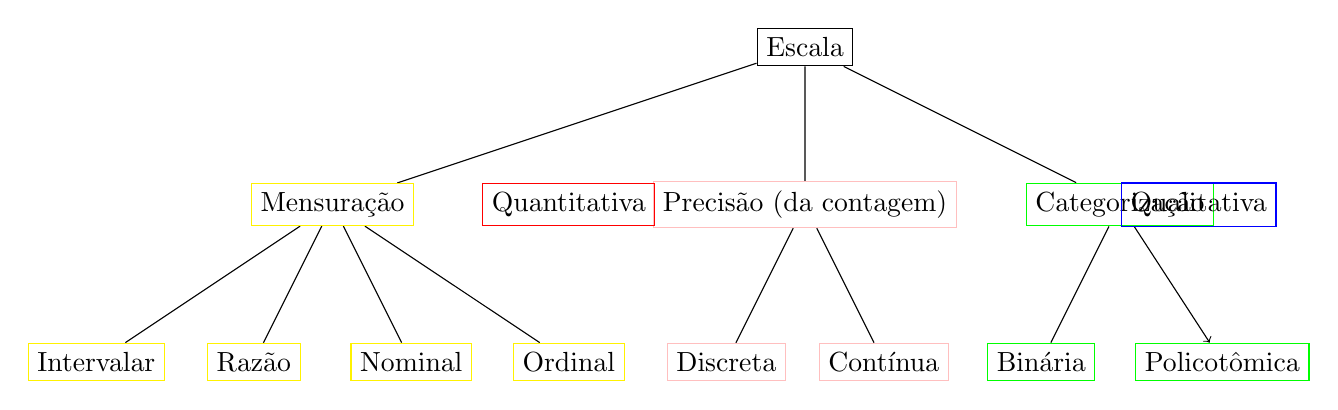
\begin{tikzpicture}
		\draw
		node[draw] at (0,2) (esc) {Escala}
		node[draw, draw=yellow] at (-6,0) (men) {Mensuração}
		node[draw, draw=pink] at (0,0) (pre) {Precisão (da contagem)}
		node[draw, draw=green] at (4,0) (cat) {Categorização}
		node[draw, draw=yellow] at (-9,-2) (int) {Intervalar}
		node[draw, draw=yellow] at (-7,-2) (raz) {Razão}
		node[draw, draw=yellow] at (-5,-2) (nom) {Nominal}
		node[draw, draw=yellow] at (-3,-2) (ord) {Ordinal}
		node[draw, draw=pink] at (-1,-2) (dis) {Discreta}
		node[draw, draw=pink] at (1,-2) (con) {Contínua}
		node[draw, draw=green] at (3,-2) (bin) {Binária}
		node[draw, draw=green] at (5.3,-2) (pol) {Policotômica}

		node[draw, draw=red] at (-3,0) (quan) {Quantitativa}
		node[draw, draw=blue] at (5,0) (qual) {Qualitativa}

		[->] (esc) -- (men)
		[->] (esc) -- (pre)
		[->] (esc) -- (cat)
		[->] (esc) -- (men)
		[->] (men) -- (int)
		[->] (men) -- (raz)
		[->] (men) -- (nom)
		[->] (men) -- (ord)
		[->] (pre) -- (dis)
		[->] (pre) -- (con)
		[->] (cat) -- (bin)
		[->] (cat) -- (pol);
\end{tikzpicture}
	\label{figescala}
\end{figure}

\begin{figure}
	\caption{Escala de \textcolor{red}{mensuração}, \textcolor{blue}{precisão} e \textcolor{green}{categorização} das variáveis quantitativa e qualitativa}
	\centering
	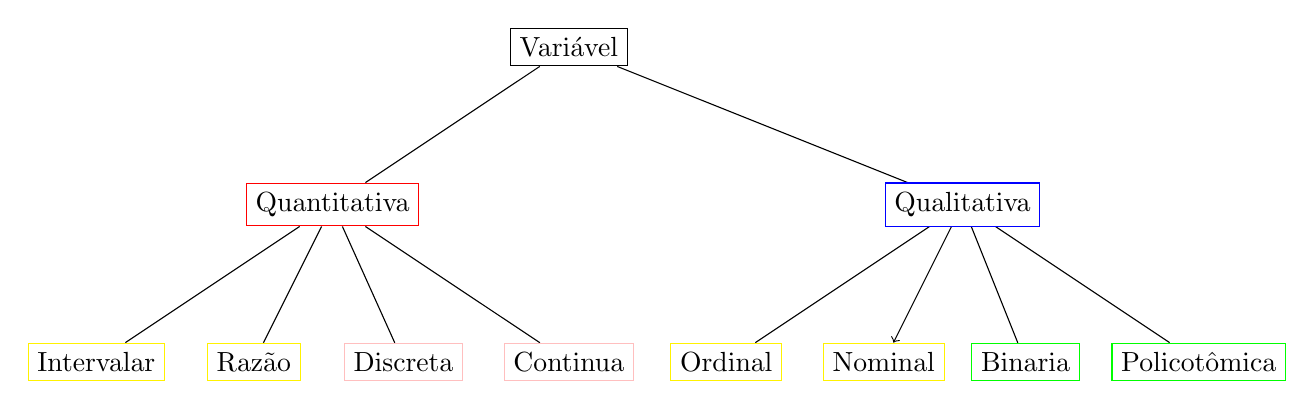
\begin{tikzpicture}
		\draw
		node[draw] at (0,2) (tipo) {Variável}
		node[draw, draw=red] at (-3,0) (quan) {Quantitativa}
		node[draw, draw=blue] at (5,0) (qual) {Qualitativa}
		node[draw, draw=yellow] at (-6,-2) (int) {Intervalar}
		node[draw, draw=yellow] at (-4,-2) (raz) {Razão}
		node[draw, draw=pink] at (-2.1,-2) (dis) {Discreta}
		node[draw, draw=pink] at (0,-2) (con) {Continua}
		node[draw, draw=yellow] at (4,-2) (nom) {Nominal}
		node[draw, draw=yellow] at (2,-2) (ord) {Ordinal}
		node[draw, draw=green] at (5.8,-2) (bin) {Binaria}
		node[draw, draw=green] at (8,-2) (pol) {Policotômica}
		[->] (tipo) -- (quan)
		[->] (tipo) -- (qual)
		[->] (quan) -- (dis)
		[->] (quan) -- (con)
		[->] (qual) -- (bin)
		[->] (qual) -- (pol)
		[->] (quan) -- (raz)
		[->] (quan) -- (int)
		[->] (qual) -- (ord)
		[->] (qual) -- (nom);
	\end{tikzpicture}
	\label{figmensuracao}
\end{figure}

Portanto se a variável for quantitativa ela somente poderá ser ou intervalar ou razão, além disso, discreta ou continua. Se ela for qualitativa, ela poderá ser ordinal ou nominal, também  binaria ou policotônica. Em outras palavras ela só terá duas dessas classificações de escala, se estivessemos lidando com cores, bastaria escolher uma opção da cor vermelha e uma da cor azul, se for quantitativa, e uma da cor vermelha e outra da cor verde se qualitativa. A Tabela~\ref{tbl:clienteclassificacaoescala} está atualizada com essa classificação das escalas.

\begin{table}
	\centering
	\caption{Classificação das variáveis, agora com as escalas.}
	\begin{tabular}{|l|l|}
		\hline
		\textbf{Nome da variável} &\textbf{Classificação} \\
		\hline
		Nome & qualitativa, nominal e policotômica  \\
		\hline
		Endereço & qualitativa, nominal e policotômica  \\
		\hline
		Telefone & qualitativa, nominal e policotômica \\
		\hline
		Estado Civil & qualitativa, nominal e binaria \\
		\hline
		Altura & quantitativa, intervalar e continua \\
		\hline
	\end{tabular}
	\label{tblclienteclassificacaoescala}
\end{table}

\subsection{Quantitativa}

Já sabemos que uma variável quantitativa é expressa geralmente (mas nem sempre) como um número, e pode ser quanto a sua escala de mensuração, intervalar ou razão. Além disso, essa variável ainda pode ser classificada em relação a sua escala de precisão, contínuo ou discreto.

Sabendo que a variável é quantitativa podemos utilizar as medidas estatísticas de posição ou localização, tais como, média, mediana, moda, quartis, decis e percentis. Também podemos utilizar as medidas de dispersão, tais como, amplitude, desvio padrão, erro-padrão e coeficiente de variação. Além disso, para uma representação visual dos gráficos podemos utilizar os gráficos do tipo linha, dispersão, histograma, ramo-e-folhas e boxplot, por fim as medidas de forma como assimetria e curtose também podem ser utilizadas\cite{favero2017manual}.

\subsubsection{Escala de precisão: Quantitativa contínua}

A  variável quantitativa pode possuir um intervalo de domínio real ou inteiro. Lembrando que o conjunto de número reais engloba os números inteiros. Geralmente essa variável é o resultado de uma medida, por exemplo, a altura dos estudantes é um dado do tipo quantitativo contínuo.

As linguagens que suportam fins estatísticos (Python, R, stata) ou as ferramentas estatísticas visuais (tais como: SPSS, JASP ou Jamovi), não são obrigadas a ter um equivalente dessa tipologia teórica. Isso depende das escolhas dos desenvolvedores e do foco da ferramenta.

Python é uma Linguagem de uso diverso, não somente estatístico. Além disso, em programação (Python) o termo variável é utilizado com um significado diferente, porém nesse capítulo, quando falamos de variável estamos nos referindo a coluna da tabela, a característica medida naquela amostra.

Vamos criar em Python uma tabela (chamado de DataFrame) que tem uma única coluna (variável) do tipo quantitativa continua. Classificamos esta coluna teoricamente em relação a escala de precisão (da contagem) como continua. Veja no código a seguir.

\begin{lstlisting}[language=Python, caption={Código que cria e exibe uma tabela em Python com uma coluna. A classificação teórica dessa variável é quantitativa continua.}]
>>> import pandas as pd
>>> dados = [1.80, 1.70, 1.50, 1.79]
>>> df = pd.DataFrame(data=dados, columns=['altura'])
>>> df
   altura
0    1.80
1    1.70
2    1.50
3    1.79
>>>
\end{lstlisting}

O Jamovi (\url{https://www.jamovi.org/}) é um software estatístico utilizado para realizar análises. No Jamovi é possível criar visualmente o conjunto de dados. Durante esse processo você informa para cada variável o \textbf{tipo de dado} e o \textbf{tipo de medida} (Figura~\ref{fig:jasp}). As opções do tipo de dado no Jamovi são: inteiro, decimal e texto. Já para o tipo de medida: nominal, ordinal, continua e ID.

\begin{figure}
\centering
\includegraphics[width=1\linewidth]{figuras/jasp}
\caption{Jamovi}
\label{figjasp}
\end{figure}

\begin{figure}

	\centering
	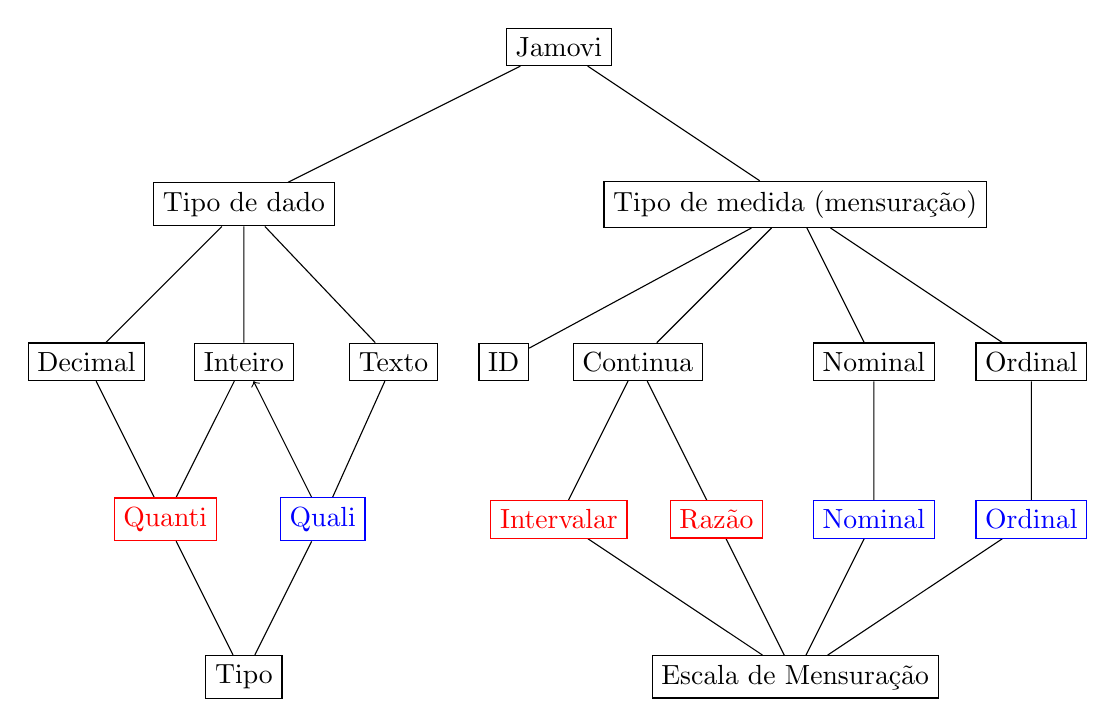
\begin{tikzpicture}
		\draw
		node[draw] at (0,2) (jamovi) {Jamovi}
		node[draw] at (-4,0) (tipd) {Tipo de dado}
		node[draw] at (3,0) (tipm) {Tipo de medida (mensuração)}
		node[draw] at (-4,-2) (int) {Inteiro}
		node[draw] at (-6,-2) (dec) {Decimal}
		node[draw] at (-2.1,-2) (tex) {Texto}
		node[draw] at (4,-2) (nom) {Nominal}
		node[draw] at (6,-2) (ord) {Ordinal}
		node[draw] at (1,-2) (con) {Continua}
		node[draw] at (-0.7,-2) (bin) {ID}

		node[draw, red] at (-5,-4) (quan) {Quanti}
		node[draw, blue] at (-3,-4) (qual) {Quali}

		node[draw, red] at (0,-4) (int_) {Intervalar}
		node[draw, red] at (2,-4) (raz_) {Razão}
		node[draw, blue] at (4,-4) (nom_) {Nominal}
		node[draw, blue] at (6,-4) (ord_) {Ordinal}

		node[draw] at (3,-6) (men) {Escala de Mensuração}
		node[draw] at (-4,-6) (tipo) {Tipo}

		[->] (jamovi) -- (tipd)
		[->] (jamovi) -- (tipm)
		[->] (tipd) -- (int)
		[->] (tipd) -- (dec)
		[->] (tipd) -- (tex)
		[->] (tipm) -- (nom)
		[->] (tipm) -- (ord)
		[->] (tipm) -- (con)
		[->] (tipm) -- (bin)

		[->] (ord) -- (ord_)
		[->] (nom) -- (nom_)
		[->] (con) -- (int_)
		[->] (con) -- (raz_)

		[->] (men) -- (int_)
		[->] (men) -- (raz_)
		[->] (men) -- (nom_)
		[->] (men) -- (ord_)

		[->] (tipo) -- (qual)
		[->] (tipo) -- (quan)
		[->] (quan) -- (dec)
		[->] (quan) -- (int)
		[->] (qual) -- (tex)
		[->] (qual) -- (int)
		;
	\end{tikzpicture}
	\caption{Jamovi Tipo de dado e tipo de medida (ou mensuração)}
	\label{figjamovi}
\end{figure}

Na tipologia teórica, uma variável do tipo quantitativa só pode ter uma escala de mensuração entre intervalar e razão, não podendo ser nominal ou ordinal, porque nominal e ordinal estão relacionados a variável qualitativa. Portanto, no Jamovi quando vc escolhe o tipo de dado decimal, automaticamente vc não consegue escolher o tipo de mensuração nominal nem ordinal. Da mesma forma quando vc escolhe o tipo texto (que equivale ao qualitativo) vc não consegue escolher intervalar ou razão, porque são as opções relacionadas a variável quantitativa.

O Jamovi, não tem a distinção entre intervalar e razão, ambas são possíveis no tipo de medida contínua.